\begin{figure}[h]
  \centering
  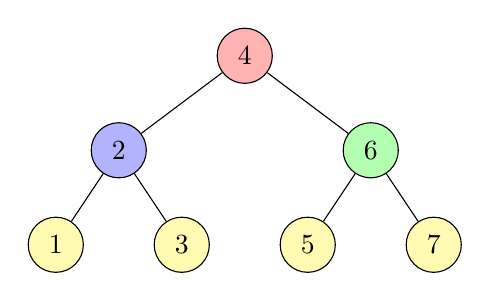
\begin{tikzpicture}[
      level distance = 12mm,
      every node/.style   = {circle, draw, minimum size=7mm, inner sep=0pt},
      level 1/.style      = {sibling distance=32mm},
      level 2/.style      = {sibling distance=16mm}
    ]
    \node[fill=red!30] {4}
      child { node[fill=blue!30] {2}
        child { node[fill=yellow!30] {1} }
        child { node[fill=yellow!30] {3} }
      }
      child { node[fill=green!30] {6}
        child { node[fill=yellow!30] {5} }
        child { node[fill=yellow!30] {7} }
      };
  \end{tikzpicture}
  \caption{Binary-search tree arranged in VEB array order.}
\end{figure}
